\documentclass[polish,envcountsect,10pt]{beamer}
    \usepackage[T1]{fontenc}
    \usepackage{fontspec}                 % żeby ustawić czcionkę na systemową (Arial)
    %\usepackage[utf8]{inputenc}
    \usepackage{polski}
    \usepackage{babel}
    \usepackage{graphicx}
    \usepackage{outlines}
    \usepackage{algorithm2e}

    \newtheorem{mdfn}{Definicja}

    \usetheme{Frankfurt}

    \title{Rozwiązywanie gier}
    \author{Michał Krakowiak}
    \subtitle{Wybrane problemy algorytmiczne i technologiczne, seminarium}
    \date{Gdańsk, 2019}

\begin{document}
    \frame{\titlepage}
    \section{Wstęp}
        \subsection{Zawartość}
            \begin{frame}
                \frametitle{Zawartość}
                \tableofcontents[pausesections]
            \end{frame}
        \subsection{Definicja gry}
            \begin{frame}
                \frametitle{Definicja gry}
                \begin{mdfn}
                    gra
                \end{mdfn}
            \end{frame}
        \subsection{Klasyfikacja gier}
            \subsubsection{Ze względu na liczbę graczy}
                \begin{frame}
                    \frametitle{Klasyfikacja ze względu na liczbę graczy}
                    \begin{outline}
                        \1 0 graczy \pause automaty \pause
                            \2 gra w życie \textit{(Conway's game of life)}\pause
                        \1 1 gracz \pause puzzle \pause
                            \2 sokoban \pause
                        \1 2 graczy \pause
                            \2 szachy \pause
                            \2 warcaby \pause
                            \2 kółko i krzyżyk
                    \end{outline}
                \end{frame}
            \subsubsection{Ze względu na złożoność}
                \begin{frame}
                    \frametitle{Klasyfikacja ze względu na złożoność}
                \end{frame}
    \section{Klasyfikacja rozwiązań}
        \subsection{Przegląd}
            \begin{frame}
                \frametitle{Klasyfikacja rozwiązań}
                \begin{itemize}
                    \item<1-> Ultra słabe
                    \item<2-> Słabe
                    \item<3-> Mocne
                \end{itemize}
            \end{frame}
        \subsection{Ultra słabe}
            \begin{frame}
                \frametitle{Rozwiązania ultra słabe}
            \end{frame}
        \subsection{Słabe}
            \begin{frame}
                \frametitle{Rozwiązania słabe}            
            \end{frame}
        \subsection{Mocne}
            \begin{frame}
                \frametitle{Rozwiązania mocne}
                Jest znany algorytm pozwalający uzyskać najlepsze ruchy z każdej pozycji (nawet jeżeli, któryś z graczy popełnił błąd)
            \end{frame}
            \begin{frame}
                \frametitle{Kółko i krzyżyk}
                \begin{figure}[H]
                    \centering
                    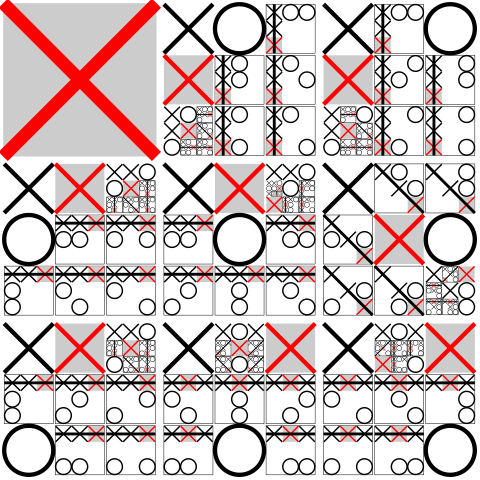
\includegraphics[width=0.55\textwidth,natwidth=480,natheight=480]{images/480px-Tictactoe-X.svg.png}
                    \caption{Optymalna gra dla X}
                \end{figure}
            \end{frame}
        \subsubsection{Kółko i krzyżyk}
            \begin{frame}
                \frametitle{Kółko i krzyżyk}
                \begin{figure}[H]
                    \centering
                    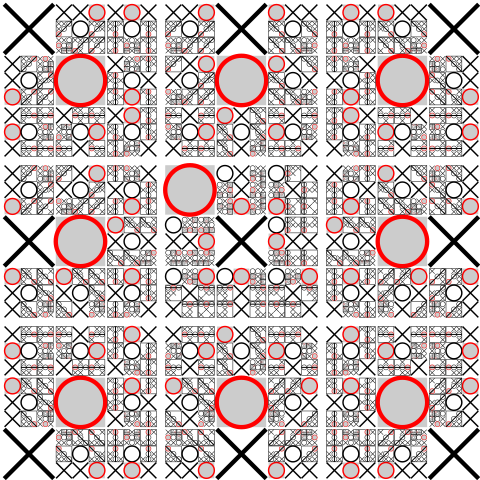
\includegraphics[width=0.55\textwidth,natwidth=480,natheight=480]{images/480px-Tictactoe-O.svg.png}
                    \caption{Optymalna gra dla O}
                \end{figure}
            \end{frame}
    \section{Szachy}
        \begin{frame}
            \frametitle{Szachy}
            \begin{figure}[]
                \centering
                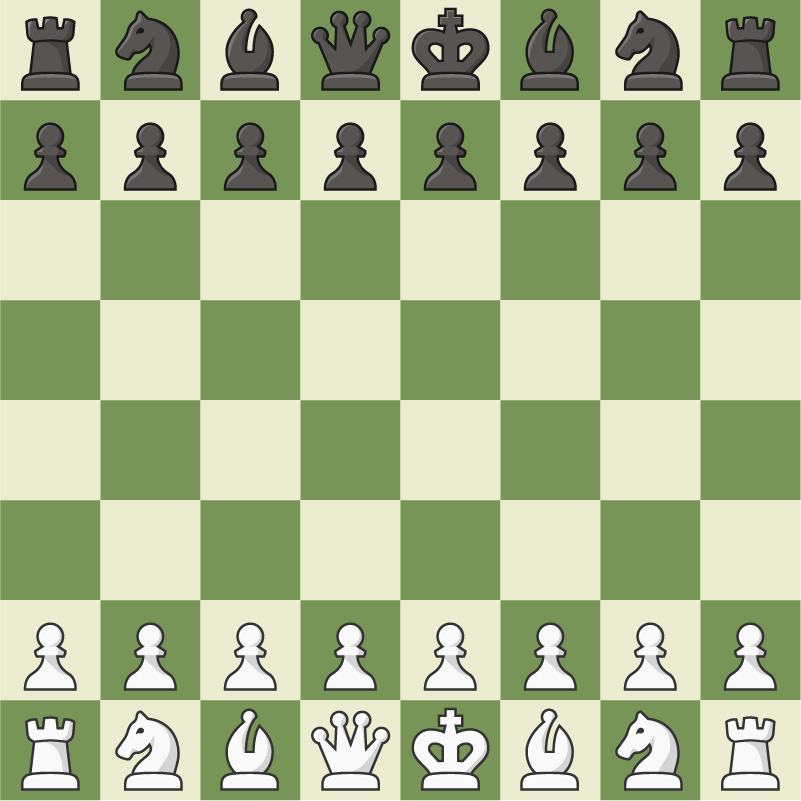
\includegraphics[width=0.55\textwidth]{images/chess.png}
                \caption{Szachy klasyczne}
            \end{figure}
        \end{frame}
        \subsection{Problematyka}
            \begin{frame}
               \frametitle{Problematyka} 
            \end{frame}
        \subsection{Minimax}
            \begin{frame}
                \begin{algorithm}[H]
                    \KwIn{test}
                    \KwOut{test}
                \caption{TEST}
                \end{algorithm}
            \end{frame}
        \subsection{NegaMax}
            \begin{frame}
                
            \end{frame}
        \subsection{Alfa-Beta Pruning}
            \begin{frame}
            \end{frame}
    \section{Literatura}
        \begin{frame}
            \frametitle{Literatura}
            \begin{thebibliography}{9}
                \bibitem{PLACEHOLDER}PLACEHOLDER
            \end{thebibliography}
        \end{frame}
\end{document}